\documentclass{article}
\usepackage[utf8]{inputenc}
\usepackage{algorithm}
\usepackage{algorithmicx}
\usepackage{algpseudocode}
\usepackage{amsmath}
\usepackage{natbib}
\usepackage{graphicx}
\usepackage{mathtools}

\title{CS6033 Assign No.8}
\author{Minghe Yang}
\date{May 2021}

\begin{document}
\renewcommand{\algorithmicrequire}{\textbf{Input:}} 
\renewcommand{\algorithmicensure}{\textbf{Output:}}
\maketitle

\section{Karger-Stein's Algorithm}
\subsection*{1.1}
\begin{figure}[h]
    \centering
    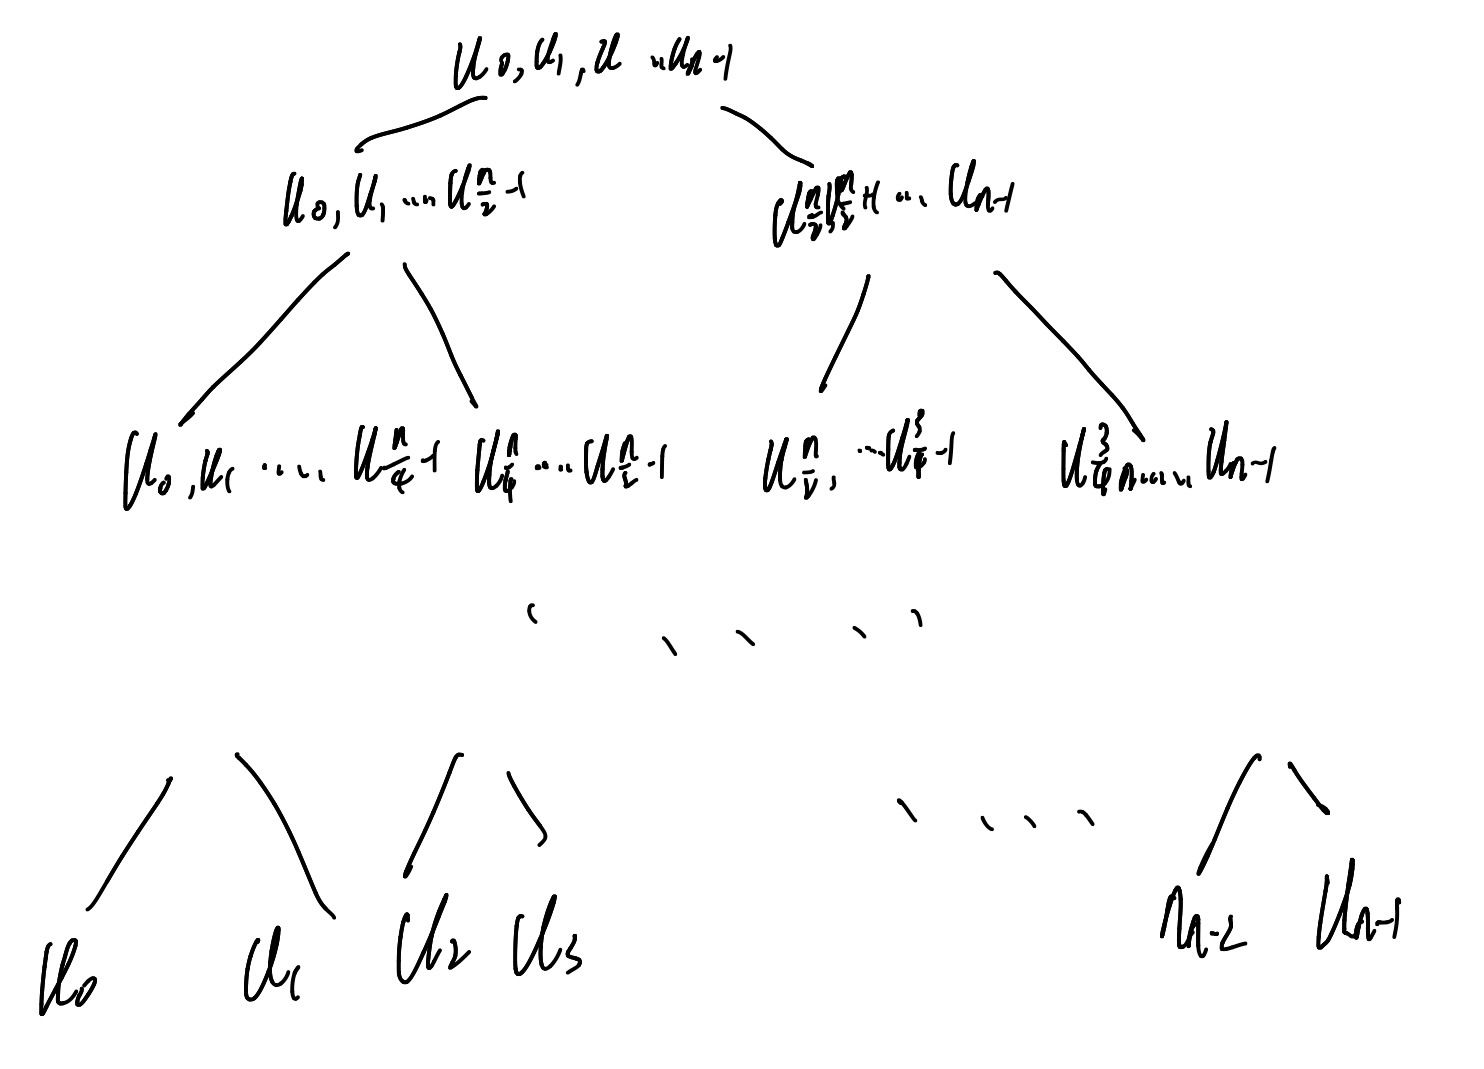
\includegraphics[scale=0.3]{h801.jpg}
    \caption{Binary Tree}
\end{figure}
\subsection*{1.2}
Firstly, $M_{0,j} = \prod_{l = 0}^{0} = m_{j+1} = m_j$.
\newline
Secondly, $M_{i+1,j} = \prod_{l = 0}^{2^{i+1}-1} = m_{j2^{i+1}+l} = M_{i, 2j}(\prod_{l = 0}^{2^i-1}m_{(2j+1)2^i+l}) = M_{i, 2j}M_{i, 2j +1}$.
\subsection*{1.3}
$M_{i,j}$ should be on $i_{th}$layer from the bottom, and $j_{th}$ node form left.
\subsection*{1.4.a}
\begin{algorithm}
    \caption{Subproduct}
    \begin{algorithmic}[1]
    \Require $n- 2^k,{u_0, u_1, \dots u_{n-1}}$ 
    \Ensure $M_{i, j}$
    \For {$i \in (0, n-1)$}
        \State $M_{0, i}\gets X-u_i$
    \EndFor
    \For {$i \in (i, k)$}
        \For {$j \in (0, 2^{k-i}-1)$}
            \State $M_{i, j}\gets M_{i-1, 2j}M_{i-1, 2j+1}$
        \EndFor
    \EndFor
    \end{algorithmic}
\end{algorithm}
\subsection*{1.4.b}
\begin{algorithm}
    \caption{Fast Multipoint Evaluation}
    \begin{algorithmic}[1]
    \Require $P, n- 2^k,{u_0, u_1, \dots u_{n-1}}, M_{i,j}$ 
    \Ensure Evaluation of $ \{{P{u_0}, P{u_1}, \dots, P(u_{n-1})}\}$
    \Function {DD}{$f, k, i$}  
		\If {$n=1$}
        \State \Return $f$  
        \EndIf
		\State $fleft\gets f\mod M_{k-1, 2i} $
        \State $fright\gets f\mod M_{k-1, 2i+1} $
		\State $lset\gets DD(fleft, k-1, 2i)$
        \State $rset\gets DD(fleft, k-1, 2i+1)$
		\State \Return{$lset, rset$}  % 返回结果 
		\EndFunction  
        \State \Return $DD(P, k, 0)$
    \end{algorithmic}
\end{algorithm}
\subsection*{1.5.a}
One layer means that f is just a constant, so returning f is true.
Suppose that is correct in k-1 layer, here comes kth.
\\So $P= qleft(u_i)M_{k-1, 0}+rleft(u_i)$, $P =qright(u_i)M_{k-1, 0}+rright(u_i)$.
qM term will be 0 , so the true value will be in the r term, which is evaluated in k-1 layer. So it is correct.
\subsection*{1.5.b}
From solution above, we can get that $T(n)= 2T(n/2)+M(n)$, so the complexity should be $O(M(n)\log{n})$.
\section{Part Two}
\subsection*{2.2}
$m' = \sum_{i = 0}^{n-1}(x-u_i)' \frac{m}{x-u_i}= \sum_{i=0}^{n-1}\frac{m}{X-u_i}$, Since all terms with $X-u_i$ is 0,only term remain will be $1/s_i$
\subsection*{2.3}
\begin{algorithm}
    \caption{Fast Evaluation}
    \begin{algorithmic}[1]
    \Require $ n- 2^k,{u_0, u_1, \dots u_{n-1}}, \{P(u_0), P(u_1), \dots , P(u_{n-1})\}, M_{i,j}$ 
    \Ensure P
    \Function {Multup}{$f, k, i$}  
		\If {$n=1$}
        \State \Return $y$  
        \EndIf
		\State $fleft\gets Multup(fleft, k-1, 2i)$
        \State $fright\gets Multup(fright, k-1, 2i+1)$
		\State \Return{$fleft\times M_{k,1}, fright\times M_{k, 0}$}  % 返回结果 
		\EndFunction  
        \State \Return $Multup(P, k, 0)$
    \end{algorithmic}
\end{algorithm}
\subsection*{2.5}
It might be correct, while needs much space for calculation.
\section{Critical Thinking}
\subsection*{2.2}
From the first line we can get, $x\times y$ is not equal to two primes numbers, and have two or more complexities.
\\Form the second part we can get, $x+ y$ is odd, and also have two or more combinations.
\\From Goldbach conjecture, all even numbers will be excluded from $x+y$, so all possible values will be $11, 17, 23, 29, 37, 41, 47, 51, 53, 57, 59, 65, 67, 71, 77, 79, 83, 87, 89, 93, 95, 97$.
\\Number like 27 and 35 should not be in the list, since it can be dived into to prime numbers.
Also, if S2 know exact answer, the S1 should delete one wrong possibility (only one). The correspond will be :
18 - 11
24 - 11
28 - 11
50 - 27
52 - 17
54 - 29
76 - 23
92 - 27
96 - 35
98 - 51
100 - 29
112 - 23
124 - 35
140 - 27
144 - 51.
\\From 52 - 17, we can get the correct answer(like if your get 11, there are three combinations, you can't judge, so only one combination is preferred), means the number is 13 and 4.


\end{document}
